\section*{附录：详细结果（不计入正文页数限制）}
\label{app:start}

本附录\emph{不}计入正文页数限制。它汇集证据状态表、证明与算法细节、核对偶表、支撑
表~\ref{tab:real}的逐数据集与逐场景数字、系统/基线/消融细节，以及反证。除明确标注外，每条记录
均为来自\texttt{experiments/}的独立复现。

\begin{figure}[t]
\centering
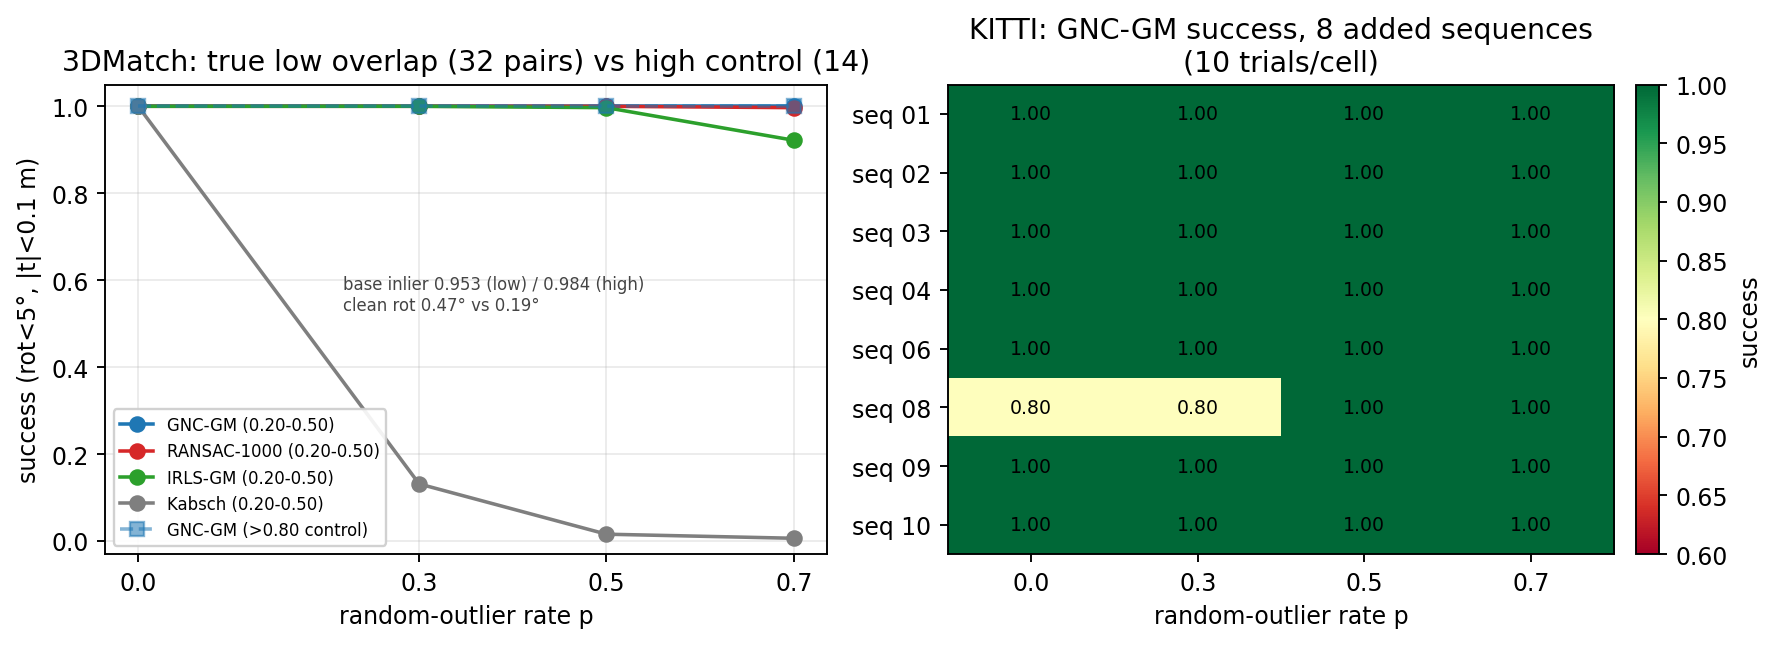
\includegraphics[width=\columnwidth]{p3_data_coverage.png}
\caption{超出原计划的数据覆盖。左：3DMatch真实低重叠带（$0.20$--$0.50$几何重叠，32个低重叠对）
与高重叠对照（14对），每格10次试验；oracle基础内点$0.953$（低） vs $0.984$（高），干净旋转
$0.47^\circ$ vs $0.19^\circ$；GNC-GM与RANSAC-1000保持$100\%$，IRLS在$p=0.7$达到$92\%$，
Kabsch崩溃到$1\%$。右：GNC-GM在新增八个KITTI odometry序列上的成功率（每格10次试验）；
seq~08是唯一真实的坏盆失效（$p=0$和$p=0.3$时为$80\%$）。来源：
\texttt{experiments/real/p3\_data\_coverage.png}。}
\label{fig:coverage}
\end{figure}

\subsection*{A. 证明、推导注记与反向算法}
\label{app:proofs}
\label{app:backward}

引理~\ref{lem:brdual}--\ref{lem:weights}、定理~\ref{thm:gnc}--\ref{thm:rhs}、
命题~\ref{prop:signflip}--\ref{prop:bound}的完整证明，Schur补恒等式、黎曼Hessian公式与存在性
构造，均维护在项目理论笔记（\texttt{theory/proofs.md}与\texttt{theory/derivations.md}）中；
数值检查在\texttt{verify/}中。正文给出适合页数预算的结果与证明梗概。具体而言：

\begin{itemize}
\item \emph{引理~\ref{lem:brdual}}：$w\mapsto we+\psi_\mu(w)$在$(0,1]$上严格凸、驻点为
  $w^*$；代入$w^*$即恢复$\rho_\mu(e)$，且盒约束是笛卡尔积，故多观测极小问题可分离。
\item \emph{引理~\ref{lem:schur}}：对联合目标在$(z,w)$上求微分得到$H_J$；利用
  $\psi''(w_i^*)=-1/\rho''(e_i^*)>0$消去$\delta w$，得到
  $H_{\mathrm{rob}}=H_{\mathrm{IRLS}}+\Delta H_{\mathrm{redesc}}$。
\item \emph{引理~\ref{lem:hessian}}：对$f\in C^2(\mathcal{M})$，限制在切空间上的欧氏Hessian与
  黎曼Hessian相差第二基本形式，对单位球面它贡献
  $-(\mathbf{q}^\top G_q)\diag(I_4,0_3)$ \cite{absil2008}。对3D--3D，
  $g_{i,q}^E=2J_i^\top W_i\mathbf{r}_i$且$J_i\mathbf{q}=2\mathbf{u}_i$，故
  $\lambda_i=\mathbf{q}^\top g_{i,q}^E=4\mathbf{u}_i^\top W_i\mathbf{r}_i$。$W_i(\theta)$扩展
  在$\partial e_i/\partial\theta$中增加
  $2\mathbf{r}_i^\top(\partial W_i/\partial\theta)\mathbf{r}_i$，并保持固定$W_i$处的Hessian
  不变。
\item \emph{命题~\ref{prop:existence}}：在$t=0$与$t=Kc^4/d^3$（$d=y_2-y_1$）处计算
  $\Phi(t)=\sum_i2\rho'(e_i)(t-y_i)$的符号，并利用$d\to\infty$时
  $H_{\mathrm{rob}}\to\lambda_\parallel(0)=2>0$。
\item \emph{命题~\ref{prop:bound}}：常数由
  $\|\partial\Phi/\partial\mathbf{y}_i\|_F\le Cc^4/(c^2+e_i)^2$、
  $\lambda_{\min}(H_{\mathrm{rob}})\ge\mu_0$、$W_i=I$时$\|\mathbf{r}_i\|^2=e_i$，以及
  $\|\rho'(e_i)g_i\|\le2\overline wc^4/\|\mathbf{r}_i\|^3$推出。
\end{itemize}

\begin{algorithm}[t]
\caption{精确反向传播（鲁棒不动点的隐式微分）}
\label{alg:backward}
\footnotesize
\begin{algorithmic}[1]
\Require 上游梯度；缓存的$z^*,w^*,e^*$
\For{$i=1$ to $N$}
  \State 计算$\mathbf{u}_i,\mathbf{r}_i,J_i,g_i^E\in\mathbb{R}^7,H_i^E\in\mathbb{R}^{7\times7}$
\EndFor
\State $G\gets\sum_i\rho'_i g_i^E$；\quad
       $H_E\gets\sum_i\big(\rho'_iH_i^E+\rho''_ig_i^Eg_i^{E,\top}\big)$
\State $B_q\gets$ $\mathbf{q}^{*\perp}$的正交基；\quad $B\gets\diag(B_q,I_3)$
\State $H_{\mathrm{rob}}\gets B^\top H_EB-\lambda_{\mathrm{rob}}\diag(I_3,0_3)$，\quad
       $\lambda_{\mathrm{rob}}=\mathbf{q}^{*\top}G_q$
\State $\mathrm{RHS}\gets\sum_i\rho'_i\,\mathrm{d}g_i/\mathrm{d}\theta
       +\sum_i\rho''_ig_i(\mathrm{d}e_i/\mathrm{d}\theta)^\top$
\State $\mathrm{d}z\gets\mathrm{solve}(H_{\mathrm{rob}},-\mathrm{RHS})$
\State 将$\mathrm{d}z$链式回传至$(\mathbf{q},\mathbf{t})$及上游损失
\end{algorithmic}
\end{algorithm}

\begin{figure}[t]
\centering
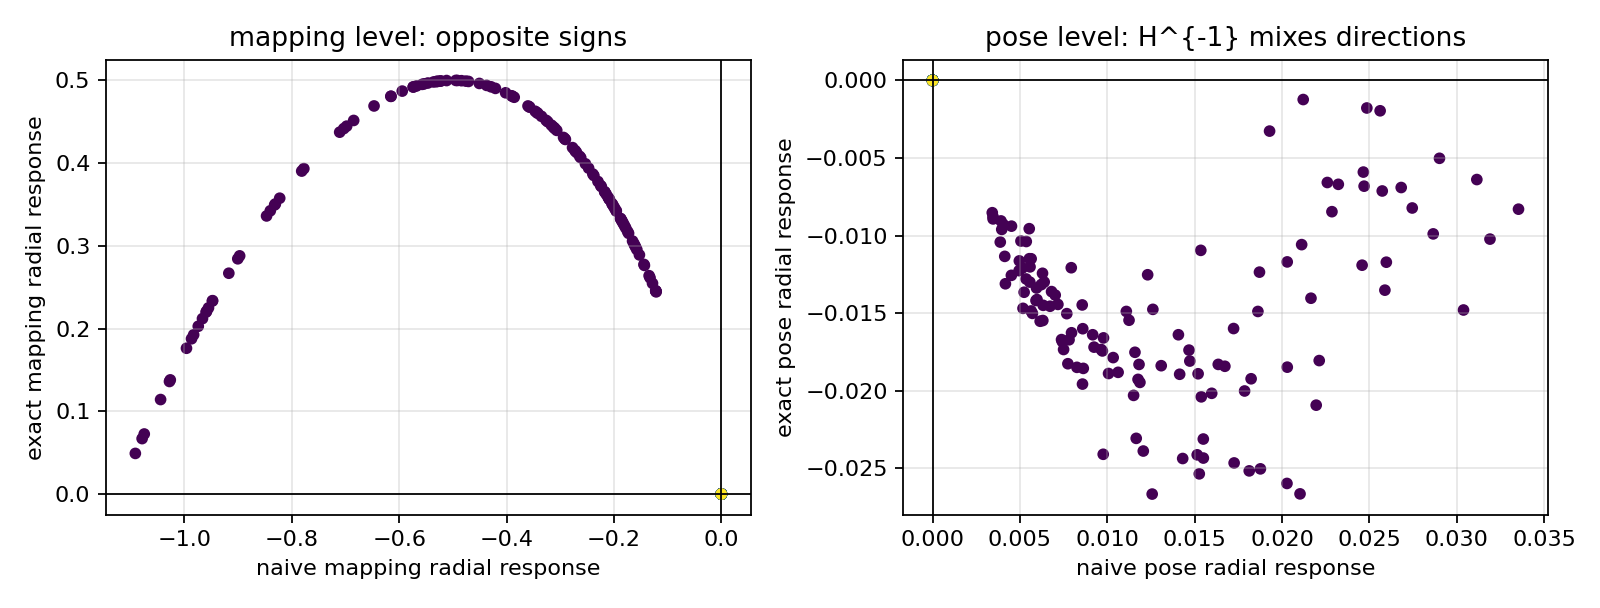
\includegraphics[width=\columnwidth]{gradient_sign.png}
\caption{命题~\ref{prop:signflip}背后的数值符号结构。左：映射级径向响应，精确 vs 冻结权重
（朴素）；当$e>c^2/3$时符号相反。右：经$H_{\mathrm{rob}}^{-1}$后的位姿级响应；逆Hessian混合
各方向，故6D符号是数值观察而非定理。来源：
\texttt{synthetic/results/gradient\_sign.png}。}
\label{fig:sign}
\end{figure}

\subsection*{B. 每条声称的证据状态}
\label{app:status}

表~\ref{tab:status}把理论、测量与受阻工程之间的边界显式化，使任何已度量行都不会被读作理论保证，
任何未来行都不会被读作结果。

\begin{table*}[t]
\caption{本文声称的证据状态（v0.4一致性检查）。产物位于
\texttt{labs/03-robust-qpeplayer/}下。}
\label{tab:status}
\centering
\scriptsize
\setlength{\tabcolsep}{3pt}
\begin{tabular}{@{}>{\raggedright\arraybackslash}p{4.2cm}
  >{\raggedright\arraybackslash}p{2.6cm}
  >{\raggedright\arraybackslash}p{6.6cm}
  >{\raggedright\arraybackslash}p{1.4cm}@{}}
\toprule
条目 & 状态 & 证据 & 章节 \\
\midrule
BR对偶、GNC不动点驻性、Schur补曲率修正、精确黎曼Hessian、一维符号翻转、存在性、
$O(\|\mathbf{r}_i\|^{-4})$界 & 新理论（证明+数值检查） & \texttt{theory/proofs.md}、
\texttt{verify/}、\texttt{synthetic/results/verify\_smoke.txt} & \S\ref{sec:method} \\
精确IFT反向 vs 中心FD（600个观测，6D） & 已度量 &
\texttt{synthetic/results/gradient\_table.json} & \S\ref{sec:experiments} \\
GNC-GM vs 固定/自适应RANSAC（随机、相干、边界外点） & 已度量（合成、ModelNet40/10、全部8个
官方3DMatch测试场景、2次KITTI raw驾驶、全部11个odometry序列） &
\texttt{synthetic/results/main\_table\_extended.json}、\texttt{real/*/results/*.json} &
\S\ref{sec:experiments} \\
端到端边界精化，NumPy与torch & 已度量的玩具诊断（GT监督，5--10个种子；非学习系统） &
\texttt{synthetic/results/e2e\_table.json}、\texttt{e2e\_torch/results/*.json} &
\S\ref{sec:experiments} \\
Theseus-GM与SDPRLayers+SCS & 仅在合成3D--3D上度量（SDPR为前向，$W_i=I$时退化为Kabsch） &
\texttt{baselines/results/baselines.json} & \S\ref{sec:experiments} \\
UTIAS In-The-Dark & 在两次白天+两次夜间前缀运行上的度量协议（复合官方GT、手写SIFT+SGBM）；
整夜/训练前端未测试 & \texttt{real/inthedark/results/} & \S\ref{sec:experiments} \\
KITTI双目回退 & 已度量的负结果（旋转可解，平移受前端限制） &
\texttt{real/kitti\_stereo/results/} & \S\ref{sec:experiments} \\
6D符号翻转陈述 & 不是定理；仅为数值观察 & \texttt{gradient\_table.json} &
\S\ref{sec:signflip} \\
通用40根QPEP多项式求解器 & 未实现（所有表格使用标量权重$4\times4$特化） &
\texttt{qpep\_gpu/qpep\_scope.md} & \S\ref{sec:experiments} \\
$4\times4$内层的GPU计时/CUDA-graph捕获 & 因Slurm GPU占用受阻；仅CPU验证 &
\texttt{qpep\_gpu/results/qpep\_gpu.json}、\texttt{logs/slurm\_gpu\_*} &
\S{}E \\
学习描述子（FCGF/Predator）、真实数据外部基线、端到端训练的In-The-Dark、完整54场景3DMatch
训练语料 & 未来工作 & --- & \S\ref{sec:notmeasured} \\
\bottomrule
\end{tabular}
\end{table*}

\subsection*{C. 核对偶}
\label{app:kernel}

表~\ref{tab:kernel}列出该层使用的BR对偶，其中$a=\mu c^2$。前向与反向在不同核之间结构完全相同：
只有$\rho_\mu'$与$\psi_\mu''$改变。TLS具有线性的$\psi$，且在$e=a$处权重不唯一；它需要GNC-TLS
调度，而不是单纯的带宽退火。

\begin{table}[t]
\caption{四种核的Black--Rangarajan对偶（$a=\mu c^2$）。来源：
\texttt{theory/derivations.md}，由\texttt{verify/}复现。}
\label{tab:kernel}
\centering
\scriptsize
\setlength{\tabcolsep}{1.5pt}
\begin{tabular}{llll}
\toprule
核 & $\rho_\mu(e)$ & $w^*=\rho_\mu'(e)$ & $\psi_\mu(w)$ \\
\midrule
Geman--McClure & $ae/(a+e)$ & $(a/(a+e))^2$ & $a(\sqrt{w}-1)^2$ \\
Cauchy & $a\log(1+e/a)$ & $a/(a+e)$ & $a(w-1-\log w)$ \\
Welsch & $a(1-e^{-e/a})$ & $e^{-e/a}$ & $a(1-w+w\log w)$ \\
TLS & $\min(e,a)$ & \shortstack[l]{$1$ (若$e<a$)\\$0$ (若$e>a$)} & $a(1-w)$ \\
\bottomrule
\end{tabular}
\end{table}

\subsection*{D. 逐数据集结果}
\label{app:datasets}

\noindent\textbf{ModelNet40/10。}表~\ref{tab:modelnet}给出汇总数字。ModelNet10使用10类共908个
测试物体，OFF网格重采样到2048点；鲁棒方法的成功率与ModelNet40最多相差$2$个百分点，中位旋转最多
相差$0.038^\circ$。

\begin{table*}[t]
\caption{均匀随机外点下的ModelNet物体点云结果，每格50次试验，$N=100$，$c=0.05$~m。来源：
\texttt{real/modelnet/results/main\_table.json}、
\texttt{real/modelnet10/results/main\_table.json}。}
\label{tab:modelnet}
\centering
\scriptsize
\setlength{\tabcolsep}{3pt}
\begin{tabular}{lcccccc}
\toprule
数据集 & GNC & RANSAC-1000 & IRLS & Kabsch & GNC ms & RANSAC ms \\
\midrule
ModelNet40 & $100\%$ $\le70\%$ & $100\%$ & $98$--$100\%$ & 崩溃$\ge50\%$ & $1.7$--$1.9$ & $53.5$--$61.5$ \\
ModelNet10 & $100\%$ $\le70\%$ & $100\%$ & $98$--$100\%$ & 崩溃$\ge50\%$ & $1.7$--$1.9$ & $53.5$--$61.5$ \\
\bottomrule
\end{tabular}
\end{table*}

\noindent\textbf{3DMatch。}表~\ref{tab:3dmatch}给出八场景汇总行、低/中/高重叠研究、更严格的
$0.20$--$0.50$带，以及两次FPFH前端审计。对全部八个官方测试场景汇总（每格20次试验），$p=0.7$
时GNC p50为$2.26$~ms，而固定1000 RANSAC为$62.6$~ms（$27.7\times$），$p=0.7$时边界中位旋转为
$0.27^\circ$ vs $0.52^\circ$。逐场景GNC p50为$2.26$--$2.36$~ms vs $62.1$--$73.4$~ms
（$27.4$--$31.1\times$），IRLS在$70\%$时为$99\%$，相干外点在$60$--$70\%$时所有方法均崩溃
（$0\%$）。重叠研究为高/中/低分箱选择24/21/20对；干净旋转为$0.18^\circ$/$0.24^\circ$/
$0.52^\circ$，但GNC与RANSAC在每个分箱、$p=0.7$时均保持$100\%$，成功差为零，$p\ge30\%$时加速
$27.7$--$30.4\times$。低分箱的中位基础内点比例仍为$0.95$。更严格的$0.20$--$0.50$几何重叠带
（每场景4个低重叠+2个匹配高重叠对，每格10次试验）的oracle基础内点为$0.953$（低）/$0.984$
（高），干净旋转$0.47^\circ$/$0.19^\circ$；GNC与RANSAC-1000在$p=0.7$时为$100\%$，IRLS为
$92\%$，Kabsch为$1\%$。低重叠减少的是可用对应的\emph{数量}，而非oracle内点比例。FPFH前端
（互为最近邻加成对距离一致性，匹配中不使用GT）在两个被审计场景上达到$80.0\%$与$67.8\%$的
自然内点率。

\begin{table*}[t]
\caption{3DMatch细节。oracle对应使用真实重叠片段上的GT映射最近邻；FPFH行使用手工前端且匹配中
不含GT（不是FCGF/Predator）。“bnd”$=$边界外点。来源：
\texttt{real/threedmatch\_full/results/full\_scenes.json}、
\texttt{overlap\_bins.json}、\texttt{overlap\_dependence.json}；
\texttt{real/threedmatch/results/descriptor.json}。}
\label{tab:3dmatch}
\centering
\scriptsize
\setlength{\tabcolsep}{3pt}
\begin{tabular}{lcccccc}
\toprule
设置 & 对数/试验数 & 干净旋转 & GNC & RANSAC-1000 & Kabsch & 加速 \\
\midrule
汇总8个测试场景，随机 & 每场景8对，每格20次 & --- & $100\%$ $\le70\%$ & $100\%$ & --- & $27.7\times$ @$70\%$ \\
汇总8个测试场景，bnd.@$70\%$ & 每场景8对，每格20次 & --- & $0.27^\circ$ & $0.52^\circ$ & --- & --- \\
重叠高 & 24对 & $0.18^\circ$ & $100\%$ @$0.7$ & $100\%$ & --- & $27.7$--$30.4\times$ \\
重叠中 & 21对 & $0.24^\circ$ & $100\%$ @$0.7$ & $100\%$ & --- & $27.7$--$30.4\times$ \\
重叠低 & 20对 & $0.52^\circ$ & $100\%$ @$0.7$ & $100\%$ & --- & $27.7$--$30.4\times$ \\
严格$0.20$--$0.50$带 & 每场景4低+2高对，每格10次 & $0.47^\circ$ / $0.19^\circ$ & $100\%$ @$0.7$ & $100\%$ & $1\%$ & --- \\
FPFH审计1 & 自然内点$80.0\%$ & --- & $100\%$ & $100\%$ & $100\%$ & --- \\
FPFH审计2 & 自然内点$67.8\%$ & --- & $100\%$ & $97\%$ & $83\%$ & --- \\
\bottomrule
\end{tabular}
\end{table*}

\noindent\textbf{KITTI。}表~\ref{tab:kitti}汇集raw驾驶与odometry行。对raw驾驶，自运动来自OXTS
（Mercator加横滚/俯仰/偏航），并用\texttt{calib\_imu\_to\_velo}映射到Velodyne；方向已验证
（drive 0001正确NN $0.100$--$0.123$~m vs 逆$0.143$--$0.183$~m；drive 0002 $0.108$--$0.140$~m
vs $0.136$--$0.269$~m）。Drive 0002精确复现drive-0001的随机与边界表格，保持相干转变
（$50\%$时GNC $40\%$ vs $35\%$，IRLS $30\%$ vs $45\%$；二者均为随机水平），并给出
$\sim21$--$23\times$的加速。阈值扫描使GNC在$c\in\{0.15,0.25,0.35\}$时保持$100\%$，其中
$c=0.25$是与$\sim0.10$~m点间距最合理的匹配。对odometry，仅从84.8~GB官方归档中按范围抓取每序列
32--33个触及帧，故全部11个序列00--10都有代表。在新增八个序列上（每格10次试验），$p=0.7$时GNC
与RANSAC-1000均为$100\%$，唯seq~08例外（$p=0$和$p=0.3$时$80\%$，真实的坏盆失效；RANSAC为
$100\%$）；11个序列汇总的成功率为$p=0/0.3/0.5/0.7$时$99/99/100/100\%$，$p\ge0.3$时固定
RANSAC/GNC运行时间比为$22.4\times$。00/05/07子集给出失效模式细节：全部18次方向检查通过
（前向NN $0.053$--$0.114$~m vs 逆$0.104$--$0.430$~m），随机成功率在$70\%$以内为$100\%$，
汇总GNC $2.8$~ms vs $73.7$~ms（$26.3\times$），$p=0.6$时相干崩溃（$p=0.5$时GNC $53\%$，
IRLS $38\%$，RANSAC $0\%$），边界$0.067^\circ$ vs $0.143^\circ$，且在
$|\mathbf{t}|=0.09$--$9.62$~m与间隔$1/2/4/8$（171个配对单元格）上GNC从未低于RANSAC。精确位姿
的干净下限（$0.042$--$0.057^\circ$）并不低于OXTS raw驾驶（$0.030$--$0.039^\circ$），故主导它
的是LiDAR采样/体素化。每序列33帧是子集，不是完整流。

\begin{table*}[t]
\caption{KITTI raw驾驶与odometry，$N=300$，$c=0.25$~m，每格20次试验（新增序列每格10次）。除
seq~08外，随机外点成功率在$70\%$以内GNC与固定1000 RANSAC均为$100\%$。来源：
\texttt{real/kitti/results/kitti.json}、\texttt{real/kitti2/results/kitti2.json}、
\texttt{real/kitti\_odom/results/kitti\_odom.json}。}
\label{tab:kitti}
\centering
\footnotesize
\setlength{\tabcolsep}{4pt}
\begin{tabular}{lcccccc}
\toprule
序列 & 帧/对 & GNC p50 & RANSAC p50 & 加速 & 相干@$50\%$ & bnd.\ 旋转 \\
\midrule
raw 0001 & 108帧，10对 & $2.7$--$2.8$~ms & $61$--$64$~ms & $\sim22\times$ & 全部$0\%$ & $0.07$--$0.09^\circ$ \\
raw 0002 & 77帧，10对 & $2.7$--$2.8$~ms & $61$--$64$~ms & $\sim21$--$23\times$ & $40/35/30/45\%$ & $0.07$--$0.09^\circ$ \\
odom 00--10 & 每个33帧，汇总 & $2.8$~ms & $73.7$~ms & $22.4\times$ & seq~08 $80\%$ @$p\le0.3$ & --- \\
odom 00/05/07 & 每个33帧 & $2.8$~ms & $73.7$~ms & $26.3\times$ & $53/38/0\%$ & $0.067/0.143^\circ$ \\
\bottomrule
\end{tabular}
\end{table*}

\noindent\textbf{In-The-Dark。}表~\ref{tab:inthedark}给出白天运行与夜间窗口。复合官方GT已在不相交
对上用双目重投影验证：前向中位$0.65$~px（run\_000002）与$0.52$~px（run\_000012），而逆为
$18.1/27.9$~px、恒等为$9.5/14.7$~px、未共轭为$21.5/31.3$~px。所有检查通过（$512\times384$
图像，左右行对齐$0.56$--$0.58$~px）。归档为905~MB，但只按范围抓取315{,}463字节的变换文件
（CRC已验证）。夜间zip（2.6--2.76~GB）未下载；只抓取了触及的窗口。运动匹配的白天对照
（run\_000002起点757，$|\mathbf{t}|=0.21$~m，旋转$0.54^\circ$）给出$85.9\%$内点与
$0.121^\circ/0.007$~m；夜间中位深度为$4.5$~m，白天为$6.7$--$7.2$~m，故夜间内点率是几何效应，
不是SIFT在黑暗中更鲁棒的证据。

\begin{table*}[t]
\caption{UTIAS In-The-Dark：两次白天运行（各15对连续图像）与两个夜间前缀窗口（各10对）；手写
SIFT+StereoSGBM前端，无训练。GT重投影列为中位像素（前向 / 逆 / 恒等 / 未共轭车辆系）。来源：
\texttt{real/inthedark/results/inthedark\_dense.json}、
\texttt{inthedark\_run12\_dense.json}、\texttt{inthedark\_night.json}、
\texttt{verify\_run\_000002.json}、\texttt{verify\_run\_000012.json}。}
\label{tab:inthedark}
\centering
\scriptsize
\setlength{\tabcolsep}{2.2pt}
\begin{tabular}{llcccccc}
\toprule
运行 & 对数 & 内点率 & 旋转 & 平移 & 成功@$0.1$~m & Kabsch & GT重投影 \\
\midrule
白天 run\_000002 & 15 & $79.4\%$ & $0.078^\circ$ & $0.020$~m & $100\%$ & $47\%$ & $0.65/18.1/9.5/21.5$ \\
白天 run\_000012 & 15 & $88.5\%$ & $0.092^\circ$ & $0.010$~m & $100\%$ & $40\%$ & $0.52/27.9/14.7/31.3$ \\
夜间 run\_000017 & 10 & $96.0\%$ & $0.135^\circ$ & $0.011$~m & $100\%$ & --- & --- \\
夜间 run\_000018 & 10 & $97.1\%$ & $0.150^\circ$ & $0.011$~m & $100\%$ & --- & --- \\
夜间稀疏 & 10 & $84.3\%$ & $0.197^\circ$ & $0.015$~m & --- & --- & --- \\
白天对照 & 10 & $85.9\%$ & $0.121^\circ$ & $0.007$~m & --- & --- & --- \\
\bottomrule
\end{tabular}
\end{table*}

\noindent\textbf{KITTI双目回退（平移为负）。}drive 0001的三十对帧，在矫正后的
\texttt{image\_02/03}（$b=0.5327$~m）上使用SIFT+亚像素+StereoSGBM，给出$17.8\%$的自然内点率
（$c=0.5$~m），每对890个对应。GNC/IRLS把旋转恢复到$0.052^\circ$，而GT内点下限为$0.071^\circ$；
但平移中位$0.70$~m vs $1.92$~m运动与$0.239$~m下限；没有方法达到$0.1$~m或$0.25$~m成功。GNC
比固定1000 RANSAC快$19.3\times$（4.21 vs 81.3~ms）。$3$--$60$~m上双目与LiDAR深度比为
$1.000$--$1.061$，排除视差尺度缺陷；残差是来自前端、遮挡与动态偏置的相干前向平移低估
（$0.63$--$0.73$）。

\subsection*{E. 系统、批处理与内层求解器}
\label{app:systems}

一个在$(B,N,3)$上向量化的numpy GNC以相同的$\mu$-调度把循环复现到旋转
$\le1.1\times10^{-14}$、平移$\le1.2\times10^{-15}$。$B=32,N=100$时批处理p50为$8.5$~ms，而
循环为$56.2$~ms（$6.60\times$）；$B=8$时加速为$2.95\times$（$N=100$）与$3.27\times$
（$N=500$）；$B=1$更慢（$0.54\times$），故对单实例循环仍是正确选择。在RTX 5090的float64
eager torch上，GPU受启动开销限制于$42.4$--$45.7$~ms：在$B\le8$时落后
（$0.04$--$0.57\times$），$B=32,N=100$时大致持平（$1.33\times$），在$B=32,N=500$
（$2.23\times$）与$B=128$（$N=100$时$4.96\times$，$N=500$时$8.24\times$）时胜出。后续探针把
这一测试扩展到静态形状$4\times4$特征求解器与CUDA-graph捕获，覆盖
$B\in\{1,8,32,128,512\}$、$N\in\{100,500\}$、float64与float32。其CPU验证发现并修复了手写
Jacobi特征求解器中的一个Givens符号缺陷（修复前：static-jacobi与NumPy最大差
$\|\Delta R\|_F\approx1.80$，且只匹配$50\%$的$\mu$-调度；修复后：$\sim10^{-16}$且$100\%$
匹配）。

\textbf{GPU支路未被度量。}2026-11-28T00:26:08，我们向\texttt{gpu}分区提交作业3184
（\texttt{probe.py}、\texttt{--gres=gpu:1}、20~min）；00:31:16时
\texttt{scontrol show job 3184}报告\texttt{JobState=PENDING}、\texttt{Reason=Resources}、
\texttt{StartTime=2026-11-28T21:23:07}（约21~h之后），而作业3151/3180/3181占着三块RTX 5090。
该作业于00:31:21被取消，随后\texttt{scontrol}报告\texttt{JobState=CANCELLED}、
\texttt{Reason=Resources}；\texttt{squeue}/\texttt{scontrol}输出在
\texttt{experiments/qpep\_gpu/\allowbreak results/logs/\allowbreak slurm\_gpu\_3184\_state.txt}中。由于没有捕获任何
计算图，我们不声称任何CUDA-graph错误，也不涉及40根QPEP求解器。

$4\times4$的Davenport/Horn内层求解器 \cite{horn1987}在数值上等价于加权Kabsch（最大
$\|R_d-R_k\|_F=1.07\times10^{-14}$，最大代价超出$9.4\times10^{-16}$），但其运行时间只在大$N$
时更优：p50比为$0.94\times$（$N=20$）、$1.02\times$（$N=100$）、$1.28\times$（$N=500$），
几何平均$1.07\times$。它是大$N$选项，不是$N=100$的默认胜出项。

\begin{figure}[t]
\centering
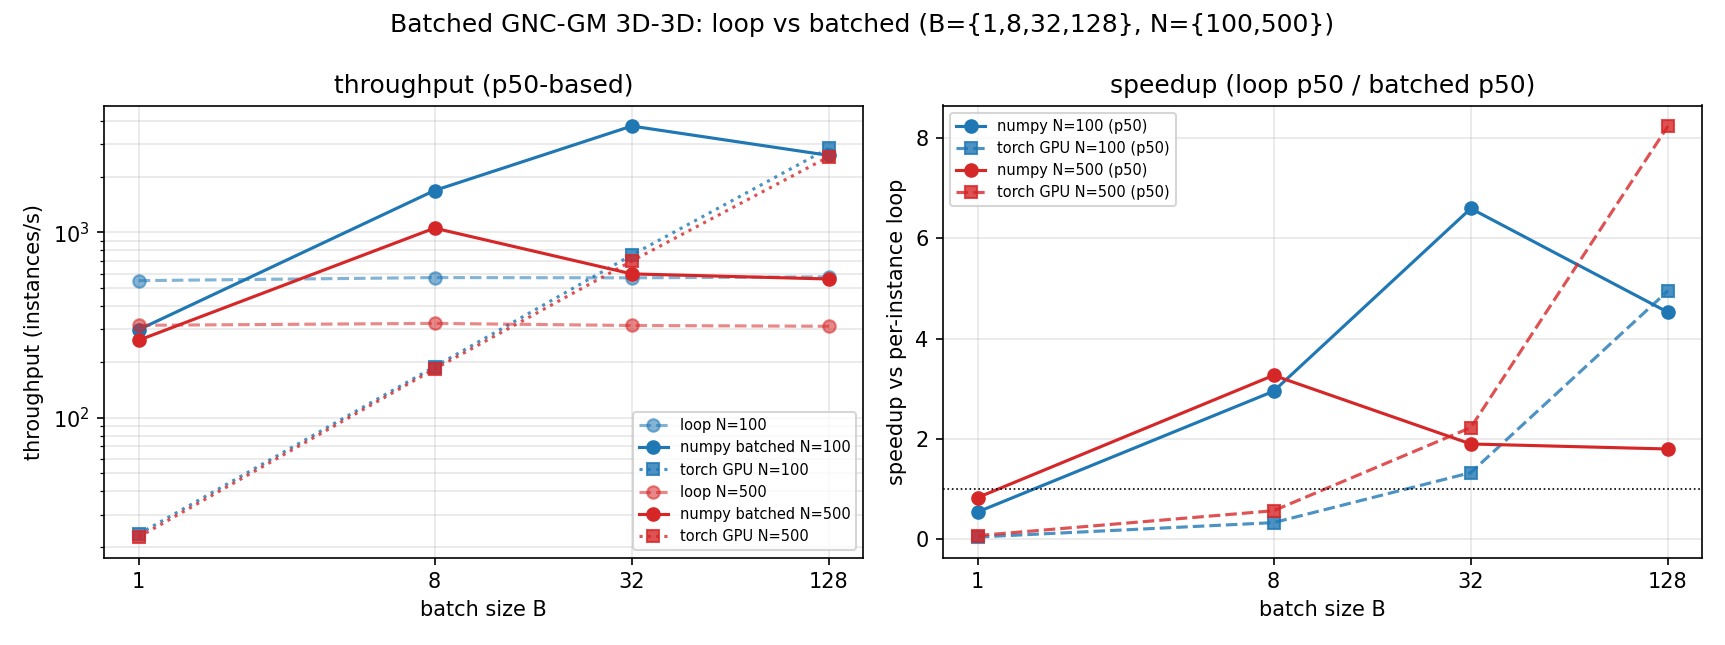
\includegraphics[width=\columnwidth]{batch_gnc.png}
\caption{$(B,N,3)$上的批处理GNC-GM：$B=\{1,8,32,128\}$与$N=\{100,500\}$的吞吐量与
循环对批处理的加速。GPU点为RTX 5090 float64 eager-torch批处理基准；它们不是受阻的静态形状
$4\times4$/CUDA-graph探针。来源：\texttt{systems/results/batch\_gnc.json}。}
\label{fig:batch}
\end{figure}

\subsection*{F. 外部基线（仅合成）}
\label{app:baselines}

Theseus 0.2.3（稠密Cholesky；无SuiteSparse头文件时\texttt{scikit-sparse}不可用）求解相同的逐点
GM目标；其Jacobian与有限差分的相对误差为$1.09\times10^{-10}$，GM代价精确一致。GT初始化下
Theseus-GM在所有$p$均$100\%$成功（局部盆检查，不是全局恢复）；随机初始化下在
$p=0/0.3/0.5/0.7$时成功率为$100/80/55/25\%$，p50为$358$--$670$~ms。在同一20个实例上，
GNC-GM在每个$p$均$100\%$，耗时$1.7$~ms，RANSAC-自适应为$100\%$、$0.2$--$14.1$~ms，而Kabsch
在$p\ge0.3$时失败。Theseus随机初始化在$p=0.3$的20次试验Wilson区间（$[0.58,0.92]$）与GNC的
$20/20$（$[0.84,1.00]$）重叠，故该差距不显著；$p=0.5/0.7$则已分离（表~\ref{tab:baselines}）。

\begin{table}[t]
\caption{合成外部基线，每个$p$有20个实例；$p=0/0.3/0.5/0.7$时的成功率（\%）与p50时间。来源：
\texttt{baselines/results/baselines.json}、\texttt{theseus.json}、
\texttt{sdpr\_forward.json}。}
\label{tab:baselines}
\centering
\scriptsize
\setlength{\tabcolsep}{1.8pt}
\begin{tabular}{lcccc}
\toprule
方法 & $p=0$ & $0.3$ & $0.5$ & $0.7$/时间 \\
\midrule
Theseus-GM，GT初值 & 100 & 100 & 100 & 100 \\
Theseus-GM，随机初值 & 100 & 80 & 55 & 25 / 358--670 \\
GNC-GM & 100 & 100 & 100 & 100 / 1.7~ms \\
RANSAC-自适应 & 100 & 100 & 100 & 100 / 0.2--14.1~ms \\
Kabsch & 100 & 失败 & 失败 & 失败 \\
SDPRLayers+SCS & 100 & 失败 & 失败 & 失败 / 8.5--13.4~ms \\
\bottomrule
\end{tabular}
\end{table}

SDPRLayers+SCS（cb3aed2处的新鲜\texttt{utiasASRL/sdprlayer}，SCS，208次前向）在数值上可用：
$0/208$次SCS异常，$8.5$--$13.4$~ms。它在$p=0$成功，但在$p\ge0.3$失败，这在无鲁棒核时符合
预期。$W_i=I$且权重为单位值时，其目标等于Kabsch：80次配对试验给出最大
$|\Delta R|=1.5\times10^{-5}$~度与最大$|\Delta t|=1.3\times10^{-9}$~m。该行是前向正确性/可用性
检查，\textbf{不是}独立的鲁棒基线；要得到有区别的SDPR，需要非单位的$W_i$（例如POLI）或
RANSAC。BPnP仅做3D--2D PnP，Pyatov等是两视图2D--2D，POLI是逐点几何估计器且未找到官方位姿
求解器代码/权重；它们都不是3D--3D基线，故没有编造任何表格。

\subsection*{G. 消融}
\label{app:ablations}

\noindent\textbf{核。}在相同的加权Kabsch内层与调度下，GM、Cauchy与Welsch在随机与边界外点上
$70\%$以内均为$100\%$（表~\ref{tab:kernelabl}）。GM在$50$--$70\%$时具有最低的边界中位旋转
（$0.199/0.229/0.340^\circ$ vs Cauchy $0.241/0.264/0.370^\circ$与Welsch
$0.220/0.268/0.392^\circ$）。没有证据支持更换默认核。

\begin{table}[t]
\caption{核消融：$p=0.5/0.6/0.7$时的边界中位旋转（度）；所有核在随机与边界外点上$70\%$以内
均为$100\%$。来源：\texttt{ablations/kernels/\allowbreak results/kernel\_ablation.json}。}
\label{tab:kernelabl}
\centering
\footnotesize
\setlength{\tabcolsep}{4pt}
\begin{tabular}{lccc}
\toprule
核 & $p=0.5$ & $p=0.6$ & $p=0.7$ \\
\midrule
GM（默认） & $0.199$ & $0.229$ & $0.340$ \\
Cauchy & $0.241$ & $0.264$ & $0.370$ \\
Welsch & $0.220$ & $0.268$ & $0.392$ \\
\bottomrule
\end{tabular}
\end{table}

\noindent\textbf{GNC调度。}扫描$\gamma\in\{1.2,1.4,1.7,2.0\}$、$\mu_0$乘子
$\{0.5,1,4\}$与精化步数$\{0,5,10\}$，在$p=0.3/0.5/0.7$时均给出$100\%$成功与相同的中位旋转；
$\gamma=2.0$比默认快$1.04$--$1.79\times$，$\gamma=1.2$慢$1.47$--$2.49\times$。默认是保守的，
不是唯一最优。

\noindent\textbf{RANSAC强度。}更强的LO-RANSAC（MSAC评分，最多五轮局部重拟合/重评分，0.999
自适应停止，上限1000）在精度上与GNC持平（中位旋转差$\le0.006^\circ$），但在每个$p$都比普通
自适应RANSAC慢$1.03$--$1.52\times$，因为最终一致性重拟合已经是同一个估计器。因此固定1000基线
在运行时间上是稻草人。

\noindent\textbf{各向异性$W_i$。}在Cholesky白化残差上使用正确的6-DoF Gauss--Newton内层求解时，
$W_i=I$与Kabsch吻合到$5.3\times10^{-13}$。标量加权Kabsch对各向异性$W_i$是\textbf{不}精确的：
在收敛的GM权重下其目标比为$1.002$--$1.007$（对角）与$1.035$--$1.088$（完整SPD），单次试验
最大为$3.80$。然而在各项同性合成噪声下，各向异性$W_i$是误设模型：完整$W$的GNC配对中位旋转
变化为$+0.055$到$+0.124^\circ$，仅在$8$--$32\%$的试验中更好，$p=0.7$时成功率为$92\%$
（单位权重：$100\%$）。精确内层求解比标量Kabsch慢$4.9$--$23\times$。故我们将其作为正确性/负
结果报告：当$W_i$确实各向异性时使用非线性内层，但不要声称在本数据上各向异性带来精度收益。

\subsection*{H. 反证}
\label{app:falsifiers}

可度量的声称都被写成可失败的形式：

\begin{itemize}
\item \textbf{精确反向。}若精确IFT Jacobian不再与精化分支上的中心有限差分吻合（相对Frobenius
  误差高于$10^{-6}$，或余弦低于$0.999$），则“精确不动点导数”的声称不成立。当前值为
  $4.9\times10^{-8}$/$3.1\times10^{-8}$（内点/边界），余弦$1.000000$。
\item \textbf{曲率修正。}若朴素冻结权重Jacobian不是边界观测上的主导误差源（例如无$\lambda$
  变体更差），则Schur补的解释无法说明测量。当前：边界上朴素$1.07$ vs 无$\lambda$
  $9.8\times10^{-4}$。
\item \textbf{符号翻转。}一维中命题即证明；数值上，若精确与朴素径向响应在$e>c^2/3$时没有
  相反符号，则6D诊断的数值前提失败。当前：$122/122$个边界与$64/64$个粗大观测翻转。
\item \textbf{前向鲁棒性。}若GNC-GM在随机外点上任一$p\in[0,0.7]$的成功率低于固定预算RANSAC，
  则“与固定预算RANSAC持平”的声称不成立。当前：在合成、ModelNet40/10、3DMatch、KITTI raw与
  odometry上持平。
\item \textbf{预算声称。}若自适应RANSAC在低$p$时比GNC慢，则所述“低$p$时更慢”的限定不成立。
  当前：GNC在$p=0.1$时慢$3.9\times$，在$p=0.7$时快$8.3\times$。
\item \textbf{可辨识性失效。}若任何方法在$60$--$70\%$相干外点下恢复了真值位姿，则模型崩溃的
  讨论有误。当前：所有方法都返回外点变换。
\item \textbf{真实数据范围。}若In-The-Dark GT在留出重投影上未能胜过逆/恒等/共轭替代，则“协议
  验证”的声称失败。当前：$0.52$--$0.65$~px vs $9.5$--$31.3$~px。
\end{itemize}
